\section{Data from Recoil energy up to 1000\,PE} 
\label{app:1000PE}
This analysis is focused on energy recoils up to 240\,keV (180\,PE) due to low statistics of NR calibration data higher energies are not considered. For completeness, the data for events with recoil energy up to 1000\,PE is presented in ~\ref{fig:eft_1000}. The data selection criteria are the same as those applied for the high-energy region.

\begin{figure}
%\centerline{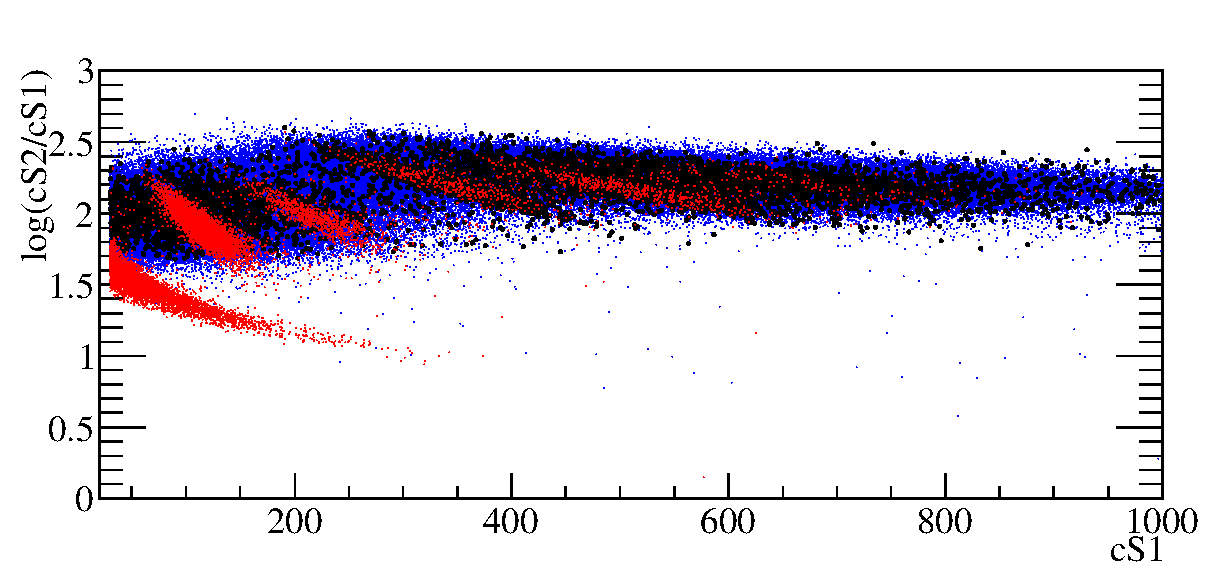
\includegraphics[width=1.\linewidth]{Figures/allDataFullScale.eps}}
Missing fig?
\caption{In blue data from ER calibration ($^{60}$Co and $^{232}$Th). In Red data from NR calibration ($^241$AmBe). In black the full dark matter search data. the two large population at ~350\,PE and ~500\,PE are the 110\,keV and 197\,keV excitation lines of $^{19}$F coming from the PTFE walls of the TPC. }
\label{fig:eft_1000}
\end{figure}  

\section{Signal model detector response table}

In this appendix we describe digital tables which can be used to construct an accurate signal model for this analysis given any input recoil spectrum $\mathrm{d}R/\mathrm{d}E$ arising from any theoretical model. A visualization of the tables is shown in Fig. \ref{fig:smeartable_highE}, and in section \ref{app:example_code} we show a simple example of how to use the supplied tables in Python. Currently we provide these tables only for the high E analysis region.

The signal model for the high E analysis region can be expressed analytically in the form:
%
\begin{align}
\label{eq:high2D}
  \frac{\mathrm{d} R}{\mathrm{d}\cSi} &= \int \! \frac{\mathrm{d}R}{\mathrm{d}E}.\epsilon_\mathrm{S1}(\cSi) .\epsilon_\mathrm{S2'}(E).p_\mathrm{S1}(\mathrm{\cSi}|E) \, \mathrm{d}E \\
  &= \int \! \frac{\mathrm{d}R}{\mathrm{d}E} G(\cSi,E) \, \mathrm{d}E
\end{align}
%
where $\epsilon_\mathrm{S1}(\cSi)$ and $\epsilon_\mathrm{S2'}(E)$ represent analysis cut efficiencies, $p_\mathrm{S1}(\mathrm{\cSi}|E)$ encodes detector effects, and $\mathrm{d}R/\mathrm{d}E$ gives the theoretically predicted nuclear recoil rate from WIMP scattering. In the second line we emphasise that all the detector and analysis effects can be encoded in a single function $G(\cSi,E)$. To make a signal prediction for the bins in our analysis this expression needs to be integrated over the appropriate range of $\cSi$ for each bin (and divided by two to account for the banding structure in $\cSiib$):
%
\begin{equation}
  R_\mathrm{bin_i} = \frac{1}{2}\int_{\mathrm{lower}_i}^{\mathrm{upper}_i} \! \frac{\mathrm{d} R}{\mathrm{d}\cSi} \, \mathrm{d}\cSi
\end{equation}
%
With some simple rearrangement this rate can be written in terms of an integral over the detector response function $G$ as follows
%
\begin{align}
  R_\mathrm{bin_i} &= \frac{1}{2}\int\frac{\mathrm{d} R}{\mathrm{d}E}\int_{\mathrm{lower}_i}^{\mathrm{upper}_i} \! G(\cSi,E) \, \mathrm{d}\cSi \, \mathrm{d}E \\
 &= \int\frac{\mathrm{d} R}{\mathrm{d}E} G'_i(E) \mathrm{d}E
\end{align}
%
where in the last line we absorb the factor of $1/2$ into the definition of $G'_i$. We see here that the signal rate for each bin can be expressed as an integral over the recoil spectrum times a detector response function $G'_i$ for that bin. It is these detector response functions which are shown in Fig. \ref{fig:smeartable_highE}, and which we provide digitally for use by the community (a low-resolution example is given in Table \ref{tab:smeartable_highE}). With these tables it is simple to produce a signal model for our analysis for any input theoretical recoil spectrum. The functions $G'_i$ are provided for three values of the nuisance variable $\Leff$, namely the median value and values at $\pm 1 \sigma$ in $\Leff$. From these, along with the measured background rates given in table \ref{table:BinDef}, one may construct a likelihood which accounts for uncertanities in $\Leff$, however simply using the $-1\sigma$ value produces quite an accurate prediction and is generally conservative.

Details of how to extract and use the provided $G'$ functions are given in the example of section \ref{app:example_code}. 

\begin{figure}
\centerline{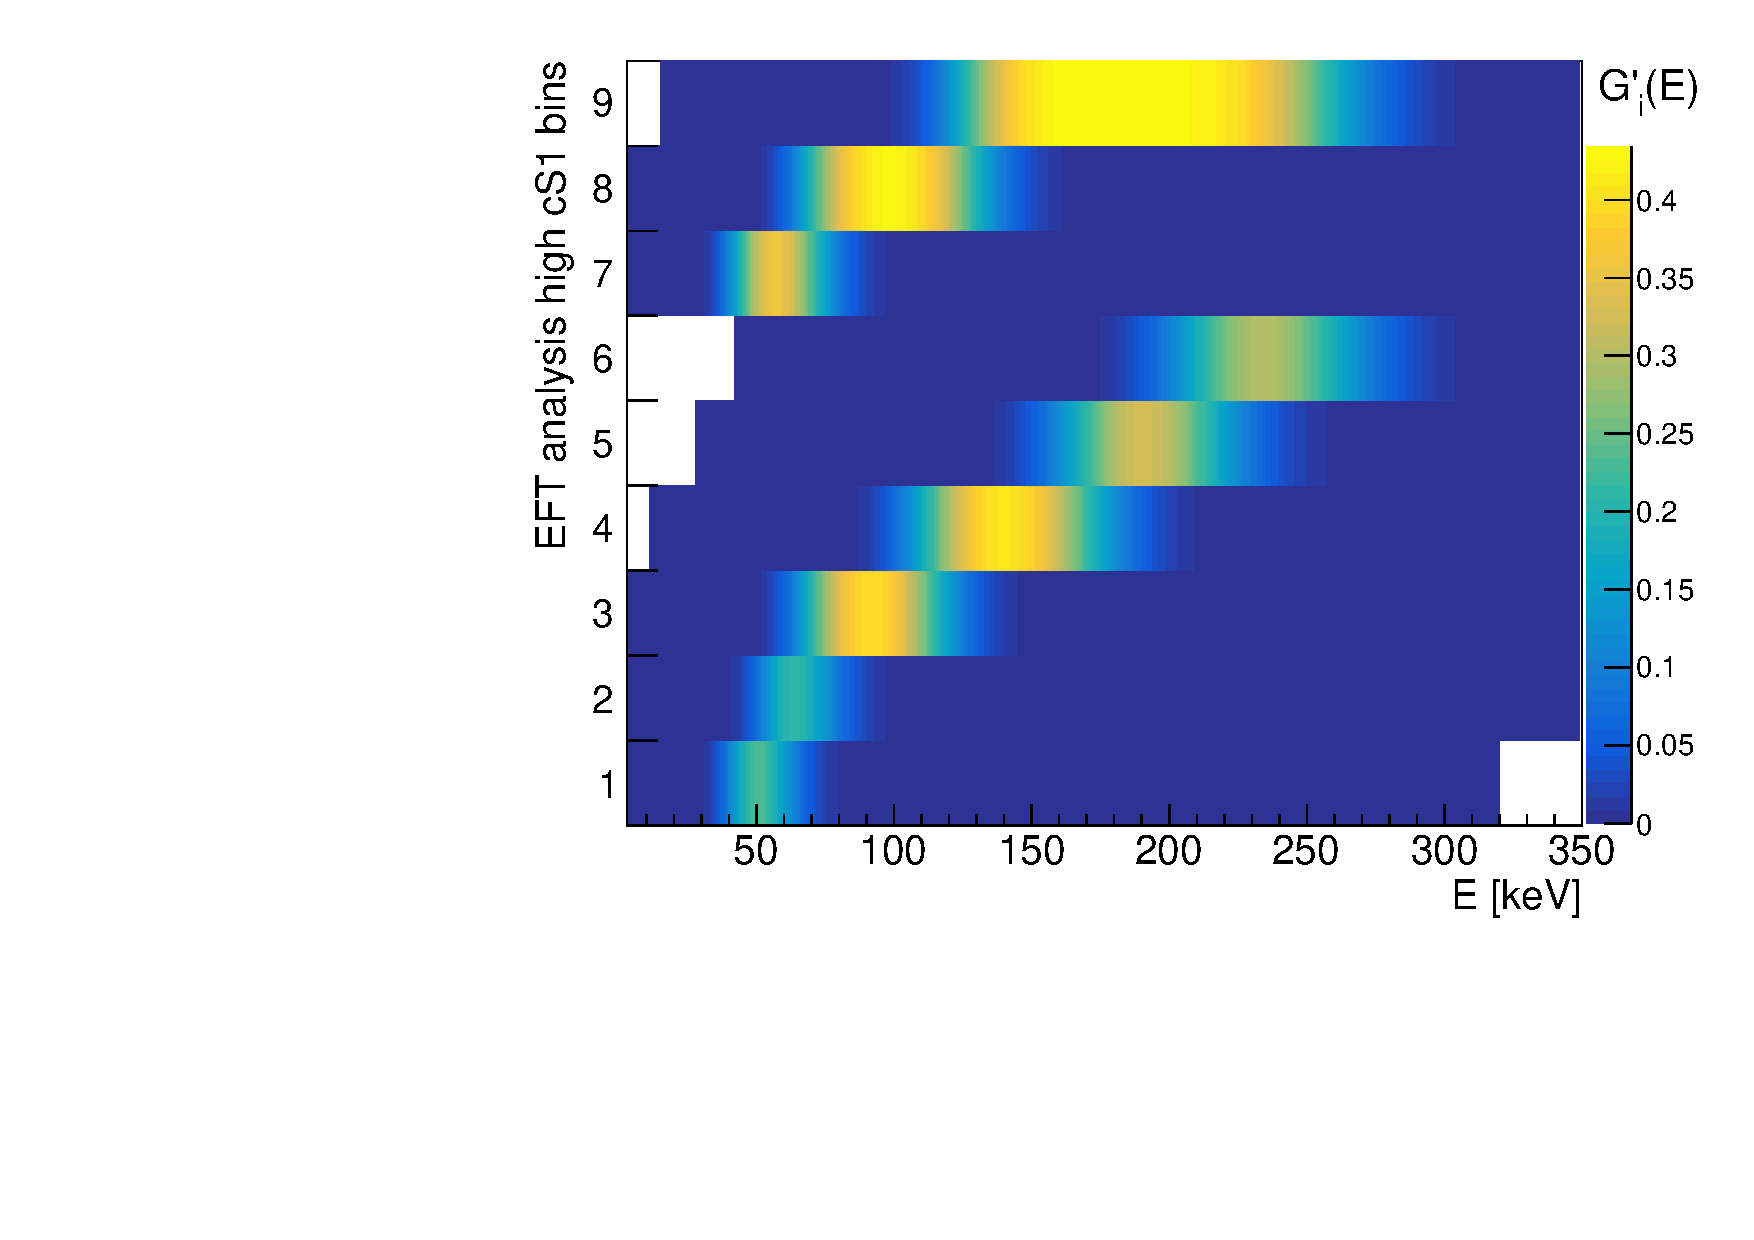
\includegraphics[width=1.\linewidth]{Figures/smeartable_highE}}
\caption{A visualization of the detector response table for $-1\sigma$ (i.e. conservative) $\Leff$, as provided in the supplementary material. The table visualization shows, on the y axis, the bins used for the high E signal region of this analysis. The $x$ axis shows recoil energies, and the colours give the probability density for a recoil of a given recoil energy to produce an event in each analysis bin. To produce a signal model for this analysis, one simply multiplies the table values by $\mathrm{d}R/\mathrm{d}E$ and integrates over $E$. The result is the predicted signal rate for each analysis bin.}
\label{fig:smeartable_highE}
\end{figure}  

\begin{table}
{
  \lstset{tabsize=4,basicstyle=\tiny\ttfamily,columns=flexible,emptylines=10000,keepspaces=true}
  \lstinputlisting{smeartable_Leff-1.dat}
}
\caption{Detector response table using $\Leff$ with constrained scaling parameter set to $-1\sigma$ value. First column gives recoil energies, subsequent columns give the values of $G'_i(E)$ for each of the 9 high E analysis bins. The sampling is in steps of 10 keV, which is too coarse to give an accurate signal model for very low WIMP masses, but is suitable for the mass range most relevant to our analysis. Higher resolution $G'_i(E)$ functions, and $G'_i(E)$ functions for other values of $\Leff$, are given in supplementary material \BenComment{give URL}. 
\label{tab:smeartable_highE}
}
\end{table}  
%\newpage
\subsection{Example code}
\label{app:example_code}
\begin{lstlisting}
import numpy as np
from numpy import newaxis
from scipy.interpolate import interp1d

def TrapI(x,y):
    """Simple trapezoid integration"""
    w = x[1:] - x[:-1]
    h = (y[1:] + y[:-1])/2.
    return np.sum(w*h,axis=0)

# Load detector response table
data = np.loadtxt("detector_table.dat")
E = data[:,0]; Gi = data[:,1:]

# Load test recoil spectrum (1 TeV WIMP, O6)
data = np.loadtxt("O6_1TeV.dat")
Er = data[:,0]
# Input spectra is normalised to coupling^2=1,
# rescale to something near limit (1e3)
# Also multiply in the appropriate exposure
dRdE = data[:,1] * (1e3/1.) * 224.6*34.

# Interpolate recoil spectrum to table values
# Assume spectrum zero outside data given
f_dRdE = interp1d(Er,dRdE)
dRdE_matched = f_dRdE(E)
Ri = TrapI(E[:,newaxis],Gi*dRdE_matched[:,newaxis])

for i,R in enumerate(Ri):
  print "bin {0}: rate = {1:.2g}".format(i+1,R)
\end{lstlisting}

Output:

\begin{lstlisting}
bin 1: rate = 0.081
bin 2: rate = 0.098
bin 3: rate = 0.35
bin 4: rate = 0.46
bin 5: rate = 0.29
bin 6: rate = 0.22
bin 7: rate = 0.18
bin 8: rate = 0.47
bin 9: rate = 0.84
\end{lstlisting}

%\vfill

